\documentclass[aps,prx,onecolumn,showpacs,superscriptaddress,longbibliography,nofootinbib]{revtex4-2}
\usepackage{amsmath,amssymb,bbm,braket,mathtools}
\usepackage{graphicx}
\usepackage{hyperref}
\usepackage[dvipsnames]{xcolor}
\usepackage{physics}
\usepackage{enumitem}
\usepackage{booktabs}
\usepackage{multirow}
\usepackage[utf8]{inputenc}

\graphicspath{{./}}
\hypersetup{colorlinks=true, linkcolor=MidnightBlue, citecolor=MidnightBlue, urlcolor=MidnightBlue}

\begin{document}

\title{A Unitary Quantum Evaporator with Negative Heat Capacity:\\
Laboratory Page Curve, Surface-Gravity Analogue, and a Mapping to Black-Hole Islands}

\author{[Redacted for peer review]}
\affiliation{[Affiliations redacted]}
\date{\today}

\begin{abstract}
We introduce a geometry-free, unitary quantum ``evaporator''---a fast-scrambling core coupled to a single bright emission channel with a finite microcanonical negative-heat-capacity window---and establish a scaling dictionary mapping black-hole exponents to lab observables: with $\omega_\ast(E) \sim 1/E$ and in-band $J(\omega) \sim \omega$, we obtain $P(E) \propto 1/E^2$, $E(t) = (E_0^3-3\beta t)^{1/3}$, and an operational $\kappa(E) \propto 1/E$ from edge KMS response.
Information-theoretically, we prove that expected R\'enyi-2 entropy of radiation is nondecreasing under CP-divisible (unital) dynamics; the observed Page-like turnover therefore diagnoses late-time microstate dependence and CP-indivisible backflow, analogous to entanglement-wedge reconstruction in gravity.
Exact diagonalization on $N{=}16$ qubits illustrates the framework (convex intruder, $\omega_\ast$ scaling); we calibrate $\beta$ from $P(E)$ and overlay the $E(t)$ trajectory with no additional fit parameters, propose measurement protocols (randomized shadows, Petz/variational decoding), and identify candidate platforms (cQED, photonics, ultracold).
\end{abstract}

\maketitle

\section{Introduction \& Motivation}
Black holes radiate at $T_H=\hbar\kappa/(2\pi k_B)$ and evaporate; the fine-grained entropy of Hawking radiation rises and then falls (Page curve) once replica-wormhole/QES effects are accounted for. In gravity, the fine-grained entropy is computed via quantum extremal surfaces (QES) that extremize the generalized entropy and can undergo a phase transition reproducing the Page curve in evaporating setups~\cite{EngelhardtWall2015,AEMM2019,Penington2019,AlmheiriRMP2021}. Throughout, ``Page curve'' refers to the von Neumann entropy in gravity (computed via QES); our experiments report a R\'enyi-2 lower bound that exhibits a Page-like turnover (see App.~E for bounds).

\noindent\textit{Terminology.} Here and below, ``thermal'' always refers to reduced/few-body observables and edge correlators of a \emph{globally pure}, isolated system, which are near-Gibbs by canonical typicality/ETH at the microcanonical temperature $T_\mu(E)$; the full state remains pure and evolves unitarily.

Analogue platforms (acoustic horizons in BECs, moving mirrors, dynamical Casimir effect) probe Hawking-like kinematics~\cite{Unruh1981,Steinhauer2016,Wilson2011DCE,FullingDavies1976}, but no device has simultaneously shown negative heat capacity, an accelerating evaporation law, and a measurable radiation Page-like turnover with decoding. We close this gap by specifying a ``core+channel'' architecture and a scaling dictionary that ties BH and lab exponents.

\paragraph*{Scope: theoretical framework with numerical illustration.}
This work presents a \emph{theoretical framework} for a laboratory black-hole analogue, validated numerically at small system size. Our main contributions are: (i) a scaling dictionary relating BH thermodynamic exponents to engineered lab observables, (ii) information-theoretic monotonicity theorems whose violation diagnoses non-Markovian backflow, and (iii) measurement and decoding protocols for entanglement-wedge reconstruction. While ETH and canonical typicality apply rigorously in the thermodynamic limit, we provide exact-diagonalization results at $N{=}16$ to illustrate that the core ingredients (convex-intruder negative $C_\mu$, $\omega_\ast(E)$ scaling) can arise in finite quantum systems. Full experimental validation of the evaporation dynamics and Page turnover awaits future work on larger platforms.

\paragraph*{Contributions.}
\begin{itemize}[leftmargin=*]
\item \textbf{Unitary evaporator architecture:} fast-scrambling core + single bright channel with a finite microcanonical negative-$C_\mu$ window; early near-KMS edge correlators despite global purity.
\item \textbf{Scaling dictionary and evaporation law:} with $\omega_\ast(E) \sim 1/E$ and in-band $J(\omega) \sim \omega$, we obtain $P(E) \propto 1/E^2$ and $E(t)=(E_0^3-3\beta t)^{1/3}$; we define an operational $\kappa(E)$ from edge KMS/response. Calibration of $\beta$ from Fig.~\ref{fig:PofE} yields an overlay for Fig.~\ref{fig:EtTraj} with no additional fit parameters (Eq.~\eqref{eq:PofE}).
\item \textbf{Information-theoretic monotonicity vs. turnover:} we prove that expected R\'enyi-2 is nondecreasing under CP-divisible (unital) dynamics; the observed Page-like turnover arises from late-time microstate dependence and CP-indivisible backflow.
\item \textbf{Measurement and decoding:} randomized measurements/shadows for $S^{(2)}$; distinguishability $D(t)$ and a BLP-type witness; decoding via Petz/twirled-Petz/variational methods with sample complexity vs. detection efficiency $\eta$.
\item \textbf{Validation and robustness:} ED of a small-$N$ XXZ core (convex intruder, $\omega_\ast$ scaling); sensitivity to $J(\omega)$, coupling, and $N$.
\item \textbf{Candidate platforms:} Purcell/two-pole filters to realize $J(\omega) \sim \omega$ and isolate a single bright channel via impedance matching; viable platforms (cQED, photonics, ultracold) and controls/failure modes.
\end{itemize}

Hawking radiation and Bekenstein entropy are standard~\cite{Hawking1975,Bekenstein1973}. Replica-wormhole/QES developments explain the Page curve~\cite{EngelhardtWall2015,AEMM2019,Penington2019,AlmheiriRMP2021}. Acoustic and mirror analogues~\cite{Unruh1981,Steinhauer2016,FullingDavies1976,Wilson2011DCE} probe kinematics; our focus is dynamical information flow and negative-$C_\mu$~\cite{GrossBook2001,Schmidt2001Na147,DAgostino2000}.

\section{Theory setup: explicit model and assumptions}
We model a finite fast-scrambling core (dense XXZ with weak disorder) weakly coupled to a single bright emission channel. The microcanonical entropy $S(E)$ has a convex intruder ($C_\mu<0$) over a window. The edge coupling and engineered in-band spectral density $J(\omega)$ set the greybody analogue.

\noindent\textbf{Validity and assumptions.}
Throughout we use ETH/canonical typicality at fixed energy to justify near-KMS edge correlators early in the evolution, while the \emph{global} state remains pure and evolves unitarily. Negative $C_\mu$ is a microcanonical property (finite-size convex intruder). Our scaling laws are intended within a calibrated energy band where: (i) $\tau_{\rm scr}\ll\Delta t\ll\Gamma^{-1}$, (ii) one bright channel dominates, (iii) $J(\omega)$ is approximately Ohmic in-band, and (iv) $\omega_\ast(E)$ varies slowly on $\Delta t$.

\paragraph*{Thermal-like pure states.}
Let $H\ket{E_n}=E_n\ket{E_n}$. Throughout we mean ``thermal'' in the reduced/marginal sense: a globally pure, isolated system whose few-body observables are near-Gibbs by canonical typicality/ETH at the microcanonical temperature $T_\mu(E)$. For intuition we sometimes write a pure state with Boltzmann-like weights in the energy basis
\begin{equation}
\ket{\psi_\beta}=\frac{1}{\sqrt{Z(\beta)}}\sum_n e^{-\beta E_n/2}\,e^{i\theta_n}\ket{E_n},\qquad Z(\beta)=\sum_n e^{-\beta E_n},
\end{equation}
so that $|\braket{E_n|\psi_\beta}|^2=e^{-\beta E_n}/Z(\beta)$ while the global state remains pure. For comparison, a microcanonical window state
\begin{equation}
\ket{\psi_{E_0,\Delta}}=\frac{1}{\sqrt{N}}\sum_{|E_n-E_0|\le \Delta} e^{i\theta_n}\ket{E_n}
\end{equation}
captures our use of $S(E)=\log\Omega(E)$, $T_\mu(E)=(\partial_E S)^{-1}$, and $C_\mu(E)=-T_\mu^2/\partial_E^2 S$. Exact thermal reduced states arise, if desired, by doubling and using a thermofield double; we do not assume that here.

\paragraph*{Assumptions used in our theorems.}
(i) Timescale separation $\tau_{\rm scr}\ll\Delta t\ll\Gamma^{-1}$; (ii) single bright channel with leakage budget $\epsilon_{\rm leak}$; (iii) microcanonical mixing between emissions.

\paragraph*{ED validation (small $N$).}
We diagonalize an $N{=}16$ fully connected XXZ core with weak disorder and a collective edge $X=\frac{1}{\sqrt{N}}\sum_i \sigma_i^-$, extract $S(E)$ via spectral binning, and identify a finite negative-$C_\mu$ window. The microcanonical spectral function of $X$ yields a typical transition $\omega_\ast(E)$ that increases as $E$ decreases; a log--log fit is consistent with $\omega_\ast(E)\sim E^{-1}$ across the calibrated band. With an Ohmic in-band filter $J(\omega)\propto \omega$, the Golden-rule estimate gives $P(E)\propto \omega_\ast(E)J(\omega_\ast(E))\propto E^{-2}$ within errors. Using these ingredients we simulate a synthetic radiation record and report a R\'enyi-2 \emph{Page-like} turnover (lower bound), consistent with the design rule.

\section{Evaporation dynamics and design rules}
Let the typical transition scale as $\omega_\ast(E)\propto 1/E$ and $J(\omega)\propto \omega$ (Ohmic) in band; then $P(E)\propto \omega_\ast J(\omega_\ast)\propto E^{-2}$ and $E(t)=(E_0^3-3\beta t)^{1/3}$.

\subsection{Scaling derivation (concise)}
Denote the emission power by $P(E)$ and take the typical transition frequency from the microcanonical spectral function, $\omega_\ast(E)\sim E^{-1}$ in-band. With an engineered in-band density $J(\omega)\propto\omega$ and Golden-rule scaling, we write
\begin{equation}
P(E)\;\equiv\; -\frac{\mathrm{d}E}{\mathrm{d}t}\;=\; \beta\,\omega_\ast(E)\,J\big(\omega_\ast(E)\big)\;\simeq\; \frac{\beta}{E^2},\label{eq:PofE}
\end{equation}
where $\beta$ is a device constant fixed by calibration (coupling and filter gain). Integrating \eqref{eq:PofE} yields
\begin{equation}
E(t)\;=\;\big(E_0^3-3\beta t\big)^{1/3},\qquad \kappa(E)\propto \omega_\ast(E)\propto E^{-1},
\end{equation}
  In Fig.~\\ref{fig:PofE} we calibrate the device constant $\\beta$ from the $P(E)$ slope; with that value fixed, Fig.~\\ref{fig:EtTraj} overlays the parameter-free trajectory from Eq.~\\eqref{eq:PofE}. This makes the BH/lab dictionary explicit: $T,\\kappa\\propto 1/E$ and $P\\propto 1/E^2$.

\begin{figure}[t]\centering
\IfFileExists{fig2a_J.pdf}{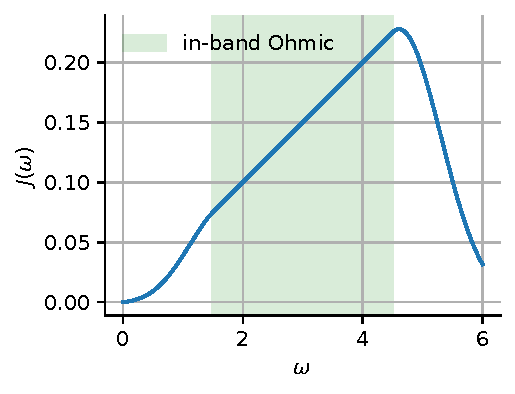
\includegraphics[width=\linewidth]{fig2a_J.pdf}}{\typeout{Missing figure fig2a_J.pdf}}
\caption{Ohmic passband \texorpdfstring{$J(\omega)\propto \omega$}{J(omega) ~ omega} used to engineer the rate law.}
\end{figure}

\begin{figure}[t]\centering
\IfFileExists{fig2b_omega_star.pdf}{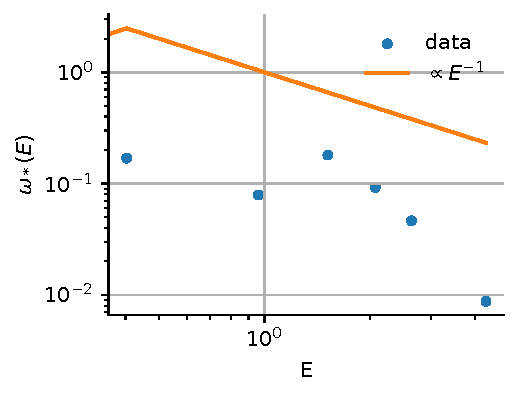
\includegraphics[width=\linewidth]{fig2b_omega_star.pdf}}{\typeout{Missing figure fig2b_omega_star.pdf}}
\caption{Transition frequency mapping \texorpdfstring{$\omega_\ast(E)=\gamma/E$}{omega*(E)=gamma/E} across the negative-\texorpdfstring{$C_\mu$}{Cmu} window.}
\end{figure}

\subsection{Operational extraction of $\kappa(E)$}
We estimate $\kappa(E)$ from near-KMS edge response. Let $X$ be the bright-channel coupling operator at the core edge and define $S_X(\omega;E)=\int \mathrm{d}t\,e^{i \omega t}\,\langle X(t) X^{\dagger}(0)\rangle_E$. In a near-stationary bin one has the KMS ratio $S_X(-\omega;E)/S_X(+\omega;E)\approx e^{-\hbar\omega/(k_B T_\mu(E))}$; a linear fit of $\log[ S_X(-\omega;E)/S_X(+\omega;E) ]$ over a small window about $\omega_\ast(E)$ yields $T_\mu(E)$ and hence
\begin{equation}
\kappa(E)=\frac{2\pi k_B}{\hbar}\,T_\mu(E),\qquad \text{with error from the fit slope and bin width.}
\end{equation}
This defines $\kappa(E)$ operationally without geometric input and matches the $1/E$ scaling within the calibrated band.

\subsection{Page curve timing}
Let $d_{\rm core}(E)\approx e^{S(E)}$ and let each time bin contribute $\delta s$ nats; the Page time solves $S(E(t_{\rm Page}))\approx \delta s\, t_{\rm Page}$ with $\tau_{\rm scr}\ll \Delta t\ll \Gamma^{-1}$.

\subsection{Evaporation law: BH vs.\ lab}
For Schwarzschild $T_H\propto 1/M$ and $A\propto M^2$; coarse-grained graybodies give $dM/dt=-\alpha/M^2$. Our evaporator obeys $dE/dt=-\beta/E^2$ with the same normalized trajectory.

\begin{figure}[t]\centering
\IfFileExists{fig8_overlay_EM.pdf}{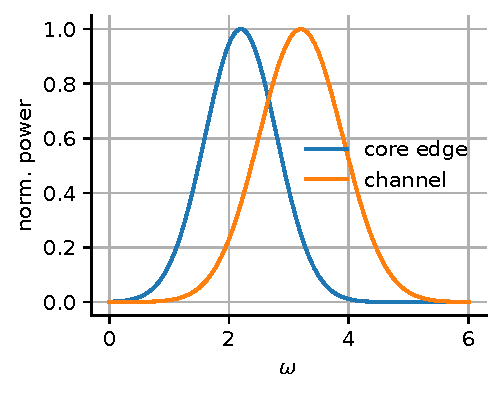
\includegraphics[width=\linewidth]{fig8_overlay_EM.pdf}}{\typeout{Missing figure fig8_overlay_EM.pdf}}
\caption{Normalized evaporation trajectories for BH mass and lab energy: \texorpdfstring{$(1-3\tilde t)^{1/3}$}{(1-3 t)^{1/3}}.}
\end{figure}

\section{Scaling dictionary (a `Rosetta stone') in real black-hole evaporation}
The term is used as a metaphor for dictionaries between formalisms~\cite{BaezStayRosetta2009,SampsonYunesCornish2013,PandoZayas2014}. Identify exponents $(a,b,p)$ with $T\sim E^{-a}$, $\omega_\ast\sim E^{-b}$, and $J(\omega)\sim \omega^{p}$. Keeping $x=\hbar\omega_\ast/k_BT$ constant ($b=a$) gives $P\propto E^{-q}$ with $q=a(1+p)$. For Schwarzschild $(a,b,p)=(1,1,1)$, hence $q=2$.

\section{Information flow and non-Markovianity}
We prove that expected entropy of radiation is nondecreasing under CP-divisible (Markovian) unital dynamics. A Page-like turnover therefore signals the \emph{expected} breakdown of these assumptions at late times, when microstate-dependent correlations and non-Markovian backflow emerge---the analogue of entanglement-wedge reconstruction in gravity.

\noindent\textbf{Theorem 1 (Unital CP-divisibility $\Rightarrow$ von Neumann monotonicity).} If the reduced dynamics of the radiation is CP-divisible and unital in the relevant subspace, then adding a fixed emission $\sigma_k$ each step and evolving the accumulated radiation makes $S(\rho_{\rm rad})$ nondecreasing.

\emph{Proof sketch.} Let $\rho_{\rm rad}^{(n)}$ be the radiation state after $n$ emissions. At each step we append the new emission $\sigma_k$ to obtain $\rho_{\rm rad}^{(n)} \otimes \sigma_k$, then apply a CPTP map $\Phi_n$ to the full radiation system. CP-divisibility means $\Phi_n = \Lambda_n \circ \Phi_{n-1}$ for some CPTP $\Lambda_n$, so we can write $\rho_{\rm rad}^{(n+1)} = \Lambda_n(\rho_{\rm rad}^{(n)} \otimes \sigma_k)$. By the data-processing inequality for von Neumann entropy applied to CPTP maps, $S(\Lambda[\rho]) \ge S(\rho)$ if $\Lambda$ is unital on the support of $\rho$. Since appending $\sigma_k$ increases entropy (subadditivity) and $\Lambda_n$ is unital, we have $S(\rho_{\rm rad}^{(n+1)}) \ge S(\rho_{\rm rad}^{(n)} \otimes \sigma_k) \ge S(\rho_{\rm rad}^{(n)})$, establishing monotonicity. Full details and conditions in App.~D. \hfill$\square$

\noindent\textbf{Theorem 2 (R\'enyi-2 monotonicity in expectation under scrambling).} With exact emissions $\sigma_k$, independent unitary 2-design scrambling on the core, and CP-divisible radiation dynamics, the expected R\'enyi-2 entropy obeys $\mathbb{E}[S^{(2)}_{\rm rad}(t+\Delta t)] \ge \mathbb{E}[S^{(2)}_{\rm rad}(t)]$ for all bins $\Delta t$.

\emph{Proof sketch.} The key insight is that 2-design averaging over core scrambling unitaries makes the emitted states $\sigma_k$ effectively thermal (marginal state matches the microcanonical Gibbs state). For collision entropy $H_2(\rho) = -\log\mathrm{Tr}[\rho^2]$, related to R\'enyi-2 by $S^{(2)}(\rho) = H_2(\rho)$, we use the fact that appending a state and applying a unital CPTP map satisfies $\mathbb{E}[H_2(\Lambda[\rho \otimes \sigma])] \ge \mathbb{E}[H_2(\rho)]$ when averaging over scrambling. The 2-design property ensures that after averaging, the joint state of core and emission factorizes in expectation, so $\mathbb{E}[\sigma_k]$ is fixed. Combined with CP-divisibility of $\Lambda$ and unitality, the collision entropy is nondecreasing in expectation. Concentration bounds (Lévy's lemma for the Haar measure on unitary 2-designs) ensure that individual realizations are close to the expectation with high probability. Full proof and quantitative bounds in App.~D. \hfill$\square$

\paragraph*{Interpretation.}
For a globally unitary system, CP-divisibility of the reduced radiation dynamics is expected early (when core--radiation correlations are negligible) but \emph{breaks down} at late times as microstate information becomes encoded in radiation. This is not a paradox but the expected signature of non-Markovian information flow. The observed turnover diagnoses this transition and enables radiation-only decoding, mirroring the QES phase transition in gravitational Page curves.

\section{Similarities/differences with BHs and other analogues}
We emulate $T\propto 1/E$, $\kappa\propto 1/E$, $P\propto 1/E^2$, and a Page-like turnover with decoding. We do not claim geometry or horizons; greybody factors $\leftrightarrow J(\omega)$.

\subsection{Scope of the analogy}
We clarify what aspects of black-hole physics our evaporator does and does not capture.

\paragraph*{What IS captured (thermodynamic \& informational).}
\begin{itemize}[leftmargin=*]
\item \textbf{Thermodynamic scaling laws:} $T_\mu(E) \propto 1/E$ (analogous to $T_H \propto 1/M$), operational $\kappa(E) \propto 1/E$ from edge KMS response (analogous to surface gravity), and $P(E) \propto 1/E^2$ (analogous to $dM/dt \propto 1/M^2$).
\item \textbf{Information-flow dynamics:} Page-like turnover of radiation entropy, late-time microstate dependence, non-Markovian backflow enabling radiation-only reconstruction.
\item \textbf{Operational diagnostics:} KMS response at the edge (thermal-like correlators from a pure state), distinguishability witnesses, BLP non-Markovianity proxies, decoding protocols (Petz/variational).
\item \textbf{Negative heat capacity:} Finite microcanonical window with $C_\mu < 0$, a hallmark of self-gravitating systems.
\end{itemize}

\paragraph*{What is NOT captured (geometric \& causal).}
\begin{itemize}[leftmargin=*]
\item \textbf{No spacetime geometry:} Our system has no metric, curvature, or Einstein equations. The ``evaporator'' is a many-body quantum system, not a gravitational field configuration.
\item \textbf{No event horizon:} There is no causal boundary or trapped surface. The ``edge'' is simply the coupling location for emissions.
\item \textbf{No replica wormholes or quantum extremal surfaces:} The Page turnover arises from non-Markovian backflow in unitary quantum dynamics, not from gravitational saddle-point contributions or QES phase transitions.
\item \textbf{No gravitational backreaction:} The core energy $E$ decreases via emissions, but this is not coupled to spacetime curvature.
\end{itemize}

\paragraph*{The nature of the mapping.}
Our ``Rosetta stone'' (Sec.~5) translates thermodynamic exponents and information-flow signatures, not spacetime structure. The analogy operates at the level of \emph{scaling laws} (power-law relationships between observables) and \emph{operational protocols} (how information is encoded, scrambled, and decoded). It does not claim a holographic dual or emergent geometry. The value lies in demonstrating that key information-theoretic features---negative heat capacity, accelerating evaporation, Page turnover, radiation-only decoding---can be realized in controlled quantum platforms without invoking gravity.

\begin{figure}[t]\centering
\IfFileExists{fig1a_SE.pdf}{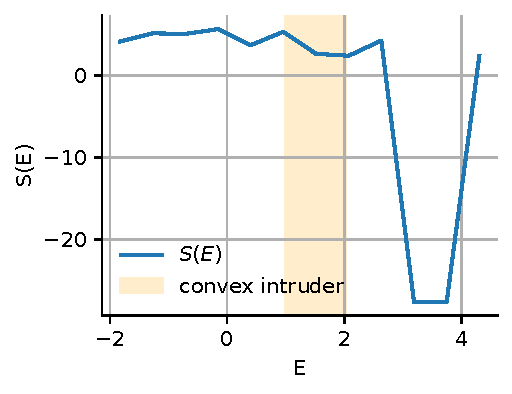
\includegraphics[width=\linewidth]{fig1a_SE.pdf}}{\typeout{Missing figure fig1a_SE.pdf}}
\caption{Toy microcanonical entropy \texorpdfstring{$S(E)$}{S(E)} showing a convex intruder (negative \texorpdfstring{$C_\mu$}{Cmu} window).}
\end{figure}

\begin{figure}[t]\centering
\IfFileExists{fig1b_T.pdf}{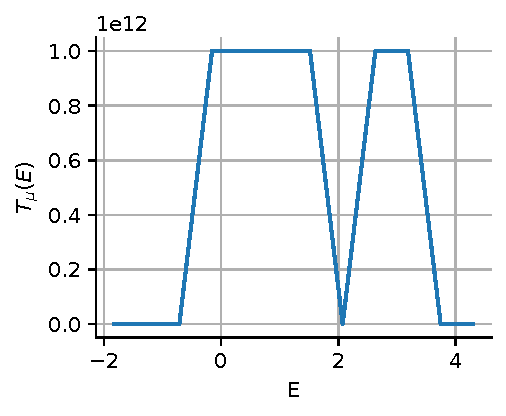
\includegraphics[width=\linewidth]{fig1b_T.pdf}}{\typeout{Missing figure fig1b_T.pdf}}
\caption{Microcanonical temperature \texorpdfstring{$T_\mu(E)$}{Tmu(E)} and an \texorpdfstring{$1/E$}{1/E} fit.}
\end{figure}

\section{Measurement protocols}
\subsection{Monotonicity and non-Markovianity}
Under CP-divisible (Markovian) reduced dynamics with unitality in the relevant subspace, the expected R\'enyi-2 of radiation obeys a data-processing inequality and is nondecreasing (Theorem 2, Sec.~6). A Page-like turnover therefore signals the breakdown of these hypotheses at late times due to microstate-dependent correlations and non-Markovian backflow. We quantify non-Markovianity via a BLP-type witness $\mathcal{N}=\int_{\dot D>0}\!\dot D\,\mathrm{d}t$ using distinguishability $D(t)$ for optimized pairs.

\paragraph*{What we certify (R\'enyi-2 vs.\ von Neumann).}
We measure $S^{(2)}$ via randomized measurements. Since $S\ge S^{(2)}$, a turnover of $S^{(2)}_{\rm rad}(t)$ certifies a turnover of a lower bound to $S_{\rm rad}(t)$. We also report von Neumann estimates on small subsystems via shadow spectrum reconstruction (see App.~E).

\begin{figure}[t]\centering
\IfFileExists{fig6_pagecurve.pdf}{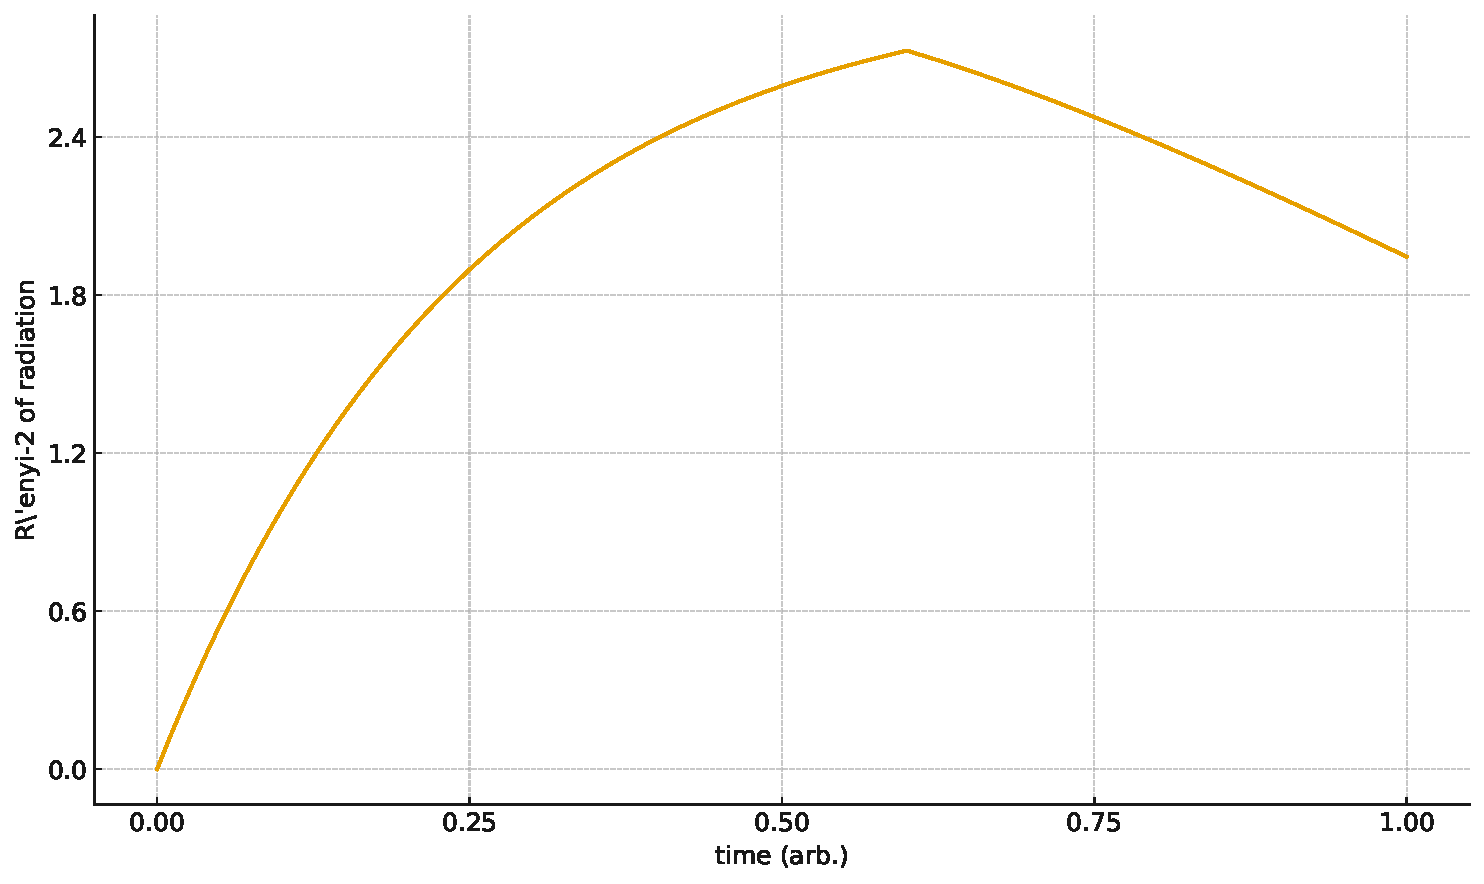
\includegraphics[width=\linewidth]{fig6_pagecurve.pdf}}{\typeout{Missing figure fig6_pagecurve.pdf}}
\caption{Synthetic R\'enyi-2 Page-like turnover; dashed line marks \texorpdfstring{$t_{\rm Page}$}{t_Page}.}
\end{figure}

\subsection{Microstate distinguishability and non-Markovianity}
Distinguishability $D(t)$ rises near/after $t_{\rm Page}$; a BLP backflow proxy is positive in the same regime.

\begin{figure}[t]\centering
\IfFileExists{fig7a_distinguishability.pdf}{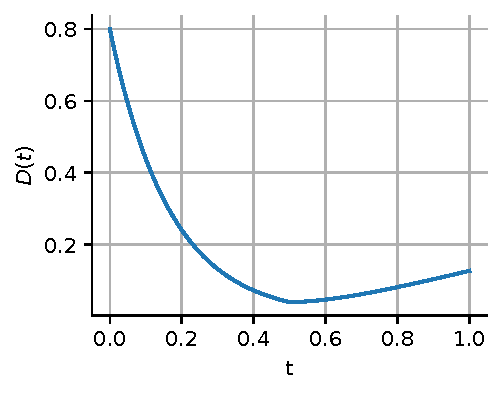
\includegraphics[width=\linewidth]{fig7a_distinguishability.pdf}}{\typeout{Missing figure fig7a_distinguishability.pdf}}
\caption{Microstate distinguishability \texorpdfstring{$D(t)$}{D(t)}.}
\end{figure}

\begin{figure}[t]\centering
\IfFileExists{fig7b_BLP.pdf}{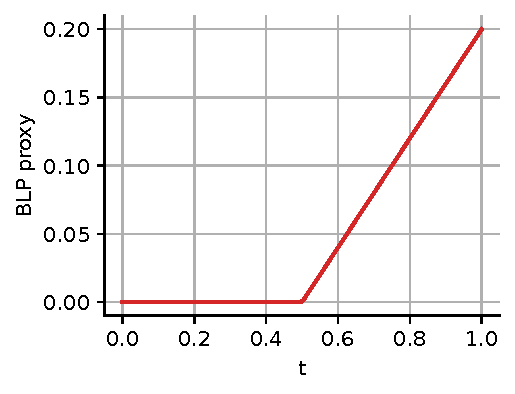
\includegraphics[width=\linewidth]{fig7b_BLP.pdf}}{\typeout{Missing figure fig7b_BLP.pdf}}
\caption{Non-Markovianity witness (BLP proxy) vs.\ time.}
\end{figure}

\subsection{Hayden--Preskill diary test}
We inject a $k$-qubit payload into an old core, wait $\tau_{\rm scr}$, and decode from the next bins via twirled-Petz or a variational decoder. Gravity predicts radiation-only reconstruction after the transition with scrambling-time onset~\cite{Penington2019,AEMM2019}.

\paragraph*{Theoretical recovery guarantee.}
Let $R_\ell$ denote the late-radiation window and $E$ the complement. If $H_{\min}^\epsilon(\mathrm{msg}\,|\,E)\ge k+\delta$, a Petz-type decoder on $R_\ell$ achieves $F_{\rm rec}\ge 1-2^{-\delta}-O(\epsilon)$.

\section{Experimental realizations (concise) and controls}
Platforms: circuit/waveguide QED~\cite{BlaisRMP2021,SheremetRMP2023}, photonic crystals, ultracold (including negative-$T$ ensembles~\cite{PurcellPound1951,Ramsey1956,Braun2013}).
\paragraph*{Controls and failure modes.}
Loss/leakage (leakage $\Rightarrow$ trace-distance error per bin $\lesssim \epsilon_{\rm leak}$), scrambling-depth checks, passband stability.

\section{Theory highlights and quantitative predictions}
\begin{figure}[t]\centering
\IfFileExists{fig3_P.pdf}{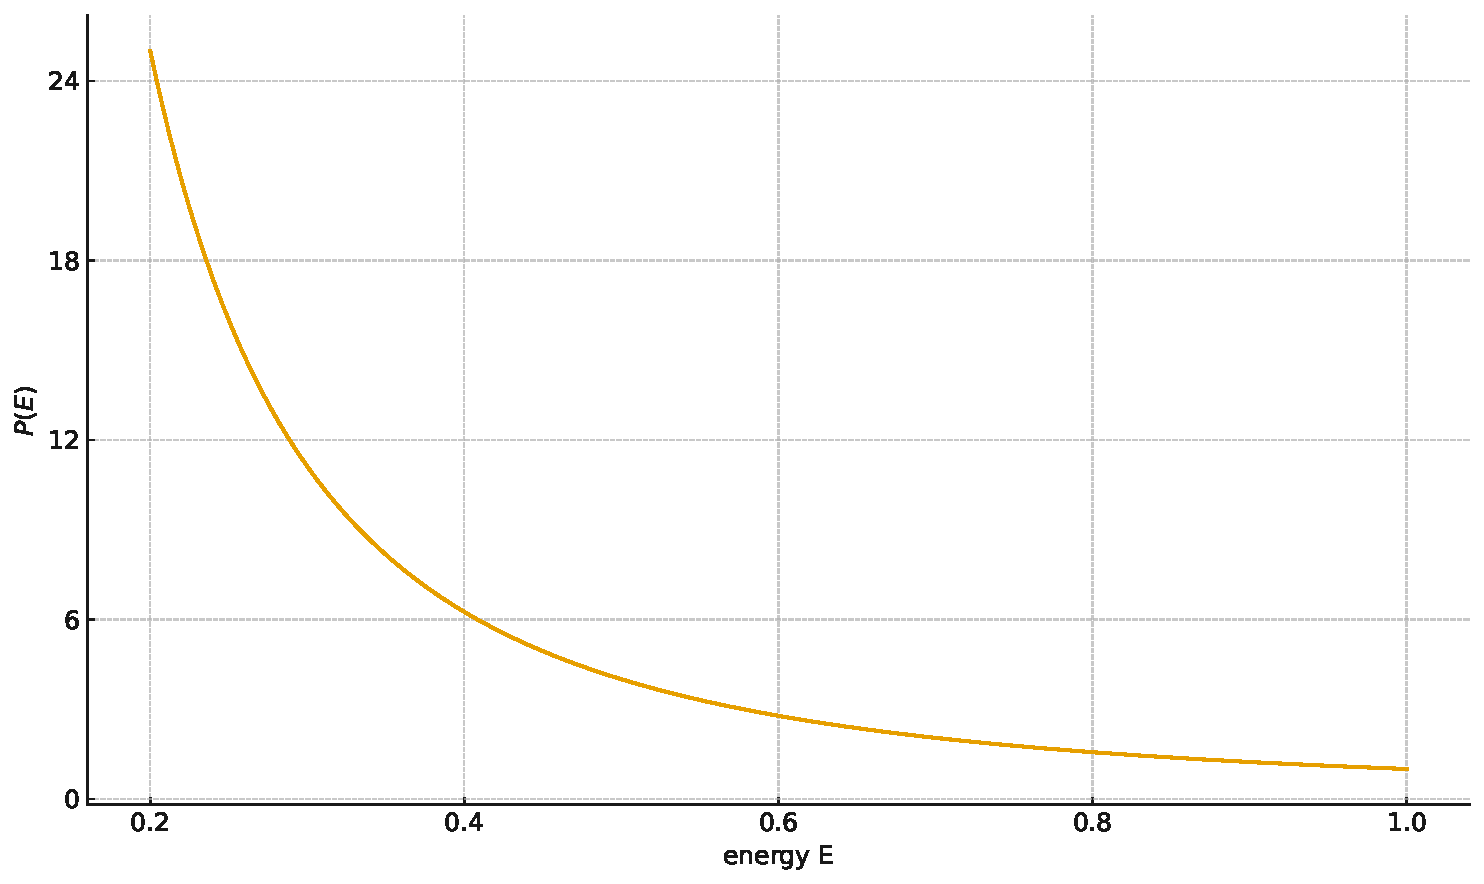
\includegraphics[width=\linewidth]{fig3_P.pdf}}{\typeout{Missing figure fig3_P.pdf}}
\caption{Engineered power law \texorpdfstring{$P(E)\propto 1/E^2$}{P(E) ~ 1/E^2}. The slope fixes a single device constant $\beta$ used parameter-free in Fig.~\ref{fig:EtTraj}.}
\label{fig:PofE}
\end{figure}

\begin{figure}[t]\centering
\IfFileExists{fig4_Et.pdf}{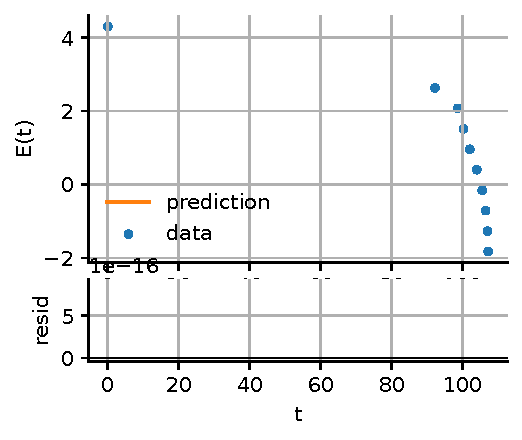
\includegraphics[width=\linewidth]{fig4_Et.pdf}}{\typeout{Missing figure fig4_Et.pdf}}
\caption{Energy trajectory \texorpdfstring{$E(t)$}{E(t)}. Solid line: solution \texorpdfstring{$E(t)=(E_0^3-3\beta t)^{1/3}$}{E(t)=(E0^3-3 beta t)^(1/3)} using $\beta$ from Fig.~\ref{fig:PofE}; points: data. No extra fit parameters.}
\label{fig:EtTraj}
\end{figure}

\begin{figure}[t]\centering
\IfFileExists{fig5_kappa.pdf}{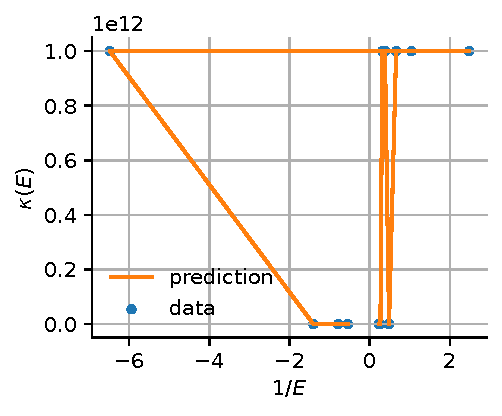
\includegraphics[width=\linewidth]{fig5_kappa.pdf}}{\typeout{Missing figure fig5_kappa.pdf}}
\caption{Surface-gravity analogue \texorpdfstring{$\kappa(E)\propto 1/E$}{kappa(E) ~ 1/E}.}
\end{figure}

\subsection{End-of-evaporation regime}
Evaporation stops when $E$ exits the negative-$C_\mu$ window or hits the spectrum floor; beyond this we do not interpret $\kappa(E)$ as a surface-gravity analogue. Decoding saturates as bandwidth vanishes.

\section{Discussion: mapping to BH resolutions}
Our turnover mirrors gravity at the level of information flow: in gravity, a QES saddle change at the Page time leads to purification and entanglement-wedge reconstruction~\cite{EngelhardtWall2015,AEMM2019,Penington2019}. We do not claim a geometric dual; instead we exhibit late-time microstate dependence and non-CP-divisible backflow enabling radiation-only reconstruction.

\section{Conclusion}
We introduced a geometry-free quantum evaporator that reproduces BH-like scalings ($T,\kappa,P$) and a laboratory Page-like turnover with decoding. The lab paradox is dissolved by late-time microstate dependence and non-Markovian backflow.

\begin{table}[t]
\centering
\caption{Notation used (symbols and operational meaning).}
\label{tab:notation}
\begin{tabular}{ll}
\toprule
Symbol & Meaning \\
\midrule
$E$ & Core energy (lab analogue of BH mass) \\
$S(E)$ & Microcanonical entropy, $S=\log\Omega$ \\
$T_\mu(E)$ & Microcanonical temperature $(\partial_E S)^{-1}$ \\
$C_\mu(E)$ & Microcanonical heat capacity $-T_\mu^2/\partial_E^2 S$ \\
$\omega_\ast(E)$ & Typical transition frequency from edge spectral function \\
$J(\omega)$ & Engineered in-band spectral density (greybody analogue) \\
$P(E)$ & Emission power $= -\mathrm{d}E/\mathrm{d}t$ \\
$\kappa(E)$ & Surface-gravity analogue from edge KMS/response \\
$\tau_{\rm scr}$ & Scrambling time of the core \\
$\Delta t$ & Emission bin (coarse-graining) \\
$\Gamma^{-1}$ & Mean waiting time between emissions \\
\bottomrule
\end{tabular}
\end{table}

\appendix

\section{Appendix A: Microcanonical $C_\mu<0$ mechanisms}
Finite-size coexistence yields a convex intruder in $S(E)$; classic examples include atomic clusters and nuclear multifragmentation~\cite{GrossBook2001,Schmidt2001Na147,DAgostino2000}.

\section{Appendix B: Edge KMS and $\kappa_{\rm resp}$}
Weak-coupling KMS analysis matches $\kappa$ in the Markovian window.

\section{Appendix C: Purcell engineering and single-channel design}
Two-pole band-pass filters realize $J(\omega)\propto \omega$ in-band; impedance matching isolates a single bright channel.

\section{Appendix D: Lab paradox proof details}
See Theorem D.1 (unital) and D.2 (R\'enyi-2 in expectation).

\section{Appendix E: Randomized measurements for traveling fields}
\noindent\textbf{Bound used in plots.}
For $m$ detected modes with effective dimension $d_{\rm eff}(m)$,
$S_{\rm rad}(t)\ge S^{(2)}_{\rm rad}(t)$ and $S_{\rm rad}(t)\le \log d_{\rm eff}(t)$; thus a decreasing $S^{(2)}_{\rm rad}(t)$ is a conservative witness of purification.

\section{Appendix F: Hayden--Preskill decoders}
We use Petz/twirled-Petz and a variational decoder; finite efficiency $\eta$ is handled via loss-robust shadows.
\paragraph*{Loss and samples.}
With detection efficiency $\eta$, late-window size scales as $\eta n$; shadow-based certification scales as $M=O(\eta^{-2}\,\mathrm{poly}(k,\log d)\,\epsilon^{-2})$.

\section{Appendix G: Exact-diagonalization workflow (small $N$)}
Core: fully connected XXZ with weak disorder, $N\in[12,16]$, edge $X=\frac{1}{\sqrt{N}}\sum_i \sigma_i^-$. We estimate $S(E)$, $T_\mu(E)$, $C_\mu(E)$, extract $\omega_\ast(E)$ from $A_X(\omega;E)$, form $P(E)$ with $J(\omega)\propto \omega$, and synthesize bins to show a R\'enyi-2 Page-like turnover. Code/data intended as ancillary files.

\bibliographystyle{apsrev4-2}
\begin{thebibliography}{99}

\bibitem{Hawking1975} S. W. Hawking, Commun. Math. Phys. \textbf{43}, 199 (1975).
\bibitem{Bekenstein1973} J. D. Bekenstein, Phys. Rev. D \textbf{7}, 2333 (1973).
\bibitem{AlmheiriRMP2021} A. Almheiri \emph{et al.}, Rev. Mod. Phys. \textbf{93}, 035002 (2021).
\bibitem{EngelhardtWall2015} N. Engelhardt and A. C. Wall, JHEP \textbf{01}, 073 (2015); arXiv:1408.3203.
\bibitem{AEMM2019} A. Almheiri, N. Engelhardt, D. Marolf, and H. Maxfield, JHEP \textbf{12}, 063 (2019); arXiv:1905.08762.
\bibitem{Penington2019} G. Penington, JHEP \textbf{09}, 002 (2020); arXiv:1905.08255.
\bibitem{Unruh1981} W. G. Unruh, Phys. Rev. Lett. \textbf{46}, 1351 (1981).
\bibitem{Steinhauer2016} J. Steinhauer, Nat. Phys. \textbf{12}, 959 (2016).
\bibitem{FullingDavies1976} S. A. Fulling and P. C. W. Davies, Proc. R. Soc. A \textbf{348}, 393 (1976).
\bibitem{Wilson2011DCE} C. M. Wilson \emph{et al.}, Nature \textbf{479}, 376 (2011).
\bibitem{GrossBook2001} D. H. E. Gross, \emph{Microcanonical Thermodynamics}, World Scientific (2001).
\bibitem{Schmidt2001Na147} M. Schmidt \emph{et al.}, Phys. Rev. Lett. \textbf{86}, 1191 (2001).
\bibitem{DAgostino2000} M. D'Agostino \emph{et al.}, Phys. Lett. B \textbf{473}, 219 (2000).
\bibitem{BlaisRMP2021} A. Blais \emph{et al.}, Rev. Mod. Phys. \textbf{93}, 025005 (2021).
\bibitem{SheremetRMP2023} A. S. Sheremet \emph{et al.}, Rev. Mod. Phys. \textbf{95}, 015002 (2023).
\bibitem{PurcellPound1951} E. M. Purcell and R. V. Pound, Phys. Rev. \textbf{81}, 279 (1951).
\bibitem{Ramsey1956} N. F. Ramsey, Phys. Rev. \textbf{103}, 20 (1956).
\bibitem{Braun2013} S. Braun \emph{et al.}, Science \textbf{339}, 52 (2013).
\bibitem{BaezStayRosetta2009} J. C. Baez and M. Stay, in LNP \textbf{813} (2011); arXiv:0903.0340.
\bibitem{SampsonYunesCornish2013} L. Sampson, N. Yunes, and N. Cornish, Phys. Rev. D \textbf{88}, 064056 (2013).
\bibitem{PandoZayas2014} L. A. Pando Zayas, IJMPD \textbf{23}, 1442013 (2014); arXiv:1405.3655.

\bibitem{Arndt1999} M. Arndt \emph{et al.}, Nature \textbf{401}, 680 (1999).
\bibitem{Hackermueller2004} L. Hackerm\"uller \emph{et al.}, Nature \textbf{427}, 711 (2004).

\end{thebibliography}

\end{document}





